% Prepared by Calvin Kent
%
% Assignment Template v19.02
%
%%% 20xx0x/MATHxxx/Crowdmark/Ax
%
\documentclass[12pt]{article} %
\usepackage{CKpreamble}
\usepackage{CKassignment}
\usepackage{tkz-euclide}
\usepackage{physunits}
\usepackage{physics}
\usepackage{lmodern}
\usepackage{tikz}
\usepackage{microtype}
\usepackage{upgreek}
\usepackage[misc]{ifsym}

%%% Maths and science packages

\usepackage{amsmath,amsthm,amssymb}
\usepackage{pgfplots}
	\usetikzlibrary{
		calc,
		patterns,
		positioning
	}
	\pgfplotsset{
		compat=1.16,
		samples=200,
		clip=false,
		my axis style/.style={
			axis x line=middle,
			axis y line=middle,
			legend pos=outer north east,
			axis line style={
				->,
			},
			legend style={
				font=\footnotesize
			},
			label style={
				font=\footnotesize
			},
			tick label style={
				font=\footnotesize
			},
			xlabel style={
				at={
					(ticklabel* cs:1)
				},
				anchor=west,
				font=\footnotesize,
			},
			ylabel style={
				at={
					(ticklabel* cs:1)
				},
				anchor=west,
				font=\footnotesize,
			},
			xlabel= $t$,
			ylabel=$x (\m)$
		},
	}
	\tikzset{
		>=stealth
	}

%%% Tables and figures packages

\usepackage{float}
\usepackage{caption}
	\captionsetup{
		format=plain,
		labelfont=bf,
		font=small,
		justification=centering
	}
	
%%% Numbers and sets

\newcommand{\E}{\mathrm{e}}

\newcommand{\tx}[1]{\text{#1}}

\begin{document}
    \pagenumbering{arabic}
    % Start of class settings ...
    \renewcommand*{\coursecode}{Physics Homework} % renew course code
    \renewcommand*{\assgnnumber}{3} % renew assignment number
    \renewcommand*{\submdate}{August 18, 2021} % renew the date
    \renewcommand*{\studentfname}{Abdullah} % Student first name
    \renewcommand*{\studentlname}{Zubair} % Student last name
    %\renewcommand*{\studentnum}{SNumber} % Student number

    \renewcommand\qedsymbol{$\blacksquare$}
    \setfigpath
    % End of class settings 
    \pagestyle{crowdmark}
    \newgeometry{left=18mm, right=18mm, top=22mm, bottom=22mm} % page is set to default values
    \fancyhfoffset[L,O]{0pt} % header orientation fixed
    % End of class settings
    %%% Note to user:
    % CTRL + F <CHANGE ME:> (without the angular brackets) in CKpreamble to specify graphics paths accordingly.
    % The command \circled[]{} accepts one optional and one mandatory argument.
    % Optional argument is for the size of the circle and mandatory argument is for its contents.
    % \circled{A} produces circled A, with size drawn for letter A. \circled[TT]{A} produces circled A with size drawn for TT.
    % https://github.com/CalvinKent/My-LaTeX
    %%%
    % Crowdmark assignment start
\begin{qstn}[1] % qnumber, qname, qpoints
    Answer the following True/False questions (\textbf{Assume [East] is positive})
    \begin{enumerate}
        \item A runner completes a $100\m$ sprint at an average speed of $50 \m / \s$.
        \begin{enumerate}[label = (\alph*)]
            \item The time it took to complete the race was $10$\s. (T / F) $\colon \textcolor{blue}{F}$
            \item If the runner wishes to complete a $1\km$ race in the same amount of time as he completed the $100\m$ race, his average speed must be $500 \m / \s$. (T / F)$\colon \textcolor{blue}{T}$
        \end{enumerate}
        \item The position v. time plot of a vehicle over the highway was similar to the plot $y = x$.
        \begin{enumerate}[label = (\alph*)]
            \item The vehicle experienced uniform motion (T / F) $\colon \textcolor{blue}{T}$
            \item The average velocity was positive (T / F) $\colon \textcolor{blue}{T}$
        \end{enumerate}
        \item The position v. time plot of a vehicle over the highway was similar to the plot $y = -4$
        \begin{enumerate}[label = (\alph*)]
            \item The vehicle experienced uniform motion (T / F)$\colon \textcolor{blue}{T}$
            \item The vehicle is [East] of the reference point (T / F)$\colon \textcolor{blue}{F}$
        \end{enumerate}
        \item Two runners compete in a race starting from $(0,0)$, runner $X$ and runner $Y$. Runner $X$ has a Pos v. Time plot similar to $y = 4x$ and Runner $Y$ has a Pos v. Time plot similar to $y = x$.
        \begin{enumerate}[label = (\alph*)]
            \item Runner $Y$ won the race (T / F) $\colon \textcolor{blue}{F}$
            \item If the race lasted $4$ seconds, then final position vector of Runner $X$ was $\vec d_X = 12\m$[East] (T / F) $\colon \textcolor{blue}{F}$
        \end{enumerate}

    \end{enumerate}

 \end{qstn}



 \begin{qstn}[2]
    Using the $x-$dimensional coordinate system, and choosing $(x \rightarrow )$ as the positive direction, I decided to track my tour around the area the other day. All position vectors are recorded relative to $(0,0)$. I \emph{began} my journey at $d_1 = + 5 \m$, then,
    \begin{itemize}
        \item $\vec d_2 = + 7\m$
        \item $\vec d_3 = -18\m$
        \item $\vec d_4 = +11\m$
    \end{itemize}
    If the tour lasted for $10\Min$, determine my average velocity as well as my average speed over the tour.
    \begin{soln}
        First we note that $\Delta t = 10\Min = (10 \times 60) \s = 600 \s$. My average velocity of the tour depends on my final and initial position vectors. My initial position vector was $\vec d_i = +5\m$ and my final position vector was $\vec d_f = \vec d_4 = +11\m$. Hence,
        $$\vec v_{av} = \frac{\Delta \vec d}{\Delta t} = \frac{+11\m - (+5\m)}{600\s} = +\frac{6}{600} \m / \s = +\frac{1}{100} \m / \s$$
        The average speed depends on the total distance traveled. To compute the total distance traveled, we return to Corollary 1.2.0.1 whereby $d = \sum_i |\overrightarrow{\Delta d}|$. Hence, we must compute each of the displacement vectors, note that we travel from $(\vec d_1 \rightarrow \vec d_2)$, $(\vec d_2 \rightarrow \vec d_3)$, $(\vec d_3 \rightarrow \vec d_4)$. This gives us an idea of how to compute the displacement vectors.
        \begin{align*}
            \Delta \vec d_1 &= \vec d_2 - \vec d_1\\
            &= +7\m - (+5\m)\\
            &= +2\m\\
            \Delta \vec d_2 &= \vec d_3 - \vec d_2\\
            &= -18\m - (+7 \m)\\
            &= -25\m\\
            \Delta \vec d_3 &= \vec d_4 - \vec d_3\\
            &= +11\m - (-18\m)\\
            &= +29 \m\\
            d &= \sum_i |\overrightarrow{\Delta d_i}|\\
            &= |\overrightarrow{\Delta d_1}| + |\overrightarrow{\Delta d_2}| + |\overrightarrow{\Delta d_3}|\\
            &= |+2\m| + |-25\m| + |+29\m|\\
            &= 2\m + 25\m + 29\m\\
            &= 56\m
        \end{align*}
        \begin{align*}
            v_{av} &= \frac{d}{\Delta t}\\
            &= \frac{56}{600} \m / \s\\
            &= \frac{7}{75} \m / \s
        \end{align*}
    \end{soln}
 \end{qstn}



\begin{qstn}[3]
    A tourist traverses $412\km[\tx{W}]$ to the Canada starting from UK. From Canada, he traverses $805\km[\tx{E}]$ to Egypt. Finally, from Egypt he traverses $98\km$[\tx{E}] to Saudi Arabia. If the journey took $2 \h$, determine his average velocity as well as his average speed (in \km / \h). 
    \begin{soln}
        We first identify the reference point to be the UK, let us assign [East] as the positive direction of motion. We must determine the initial and final position vectors relative to the UK. The initial position vector is clearly $\vec d_I = +0\m$. The final position vector will be $\vec d_{\tx{SAU rel UK}}$, to obtain this position vector we will have to preform some relative vector operations, in particular we must use proposition 1.6.1 which states that $\vec d_{\tx{C rel A}} = \vec d_{\tx{C rel B}} + \vec d_{\tx{B rel A}}$. We have the following relative position vectors,
        \begin{itemize}
            \item $\vec d_{\tx{CAD rel UK}} = -412\km$
            \item $\vec d_{\tx{EGY rel CAD}} = +805 \km$
            \item $\vec d_{\tx{SAU rel EGY}} = +98\km$
        \end{itemize}
        Observe that we can get $(SAU \rightarrow CAD)$ by the latter two position vectors and then $(SAU \rightarrow UK)$ by combining the final result with the first position vector.
        \begin{align*}
            \vec d_{\tx{SAU rel CAD}} &= \vec d_{\tx{SAU rel EGY}} + \vec d_{\tx{EGY rel CAD}}\\
            &= +98\km + (+805\km)\\
            &= +903\km\\
            \vec d_{\tx{SAU rel UK}} &= \vec d_{\tx{SAU rel CAD}} + \vec d_{\tx{CAD rel UK}}\\
            &= +903\km + (-412\km)\\
            &= +491\km\\
            \Delta \vec d &= \vec d_F - \vec d_I\\
            &= +491\km - (+0\km)\\
            &= +491\km\\
            \vec v_{av} &= \frac{\Delta \vec d}{\Delta t}\\
            &= \frac{+491\km}{2\h}\\
            &= +245.5 \km / \h = 245.5 \km/\h [\tx{E}]
        \end{align*}
        To obtain the average speed we observe that each time he "traverses", he actually displaces by that amount. Hence his displacements are,
        \begin{itemize}
            \item $(UK \rightarrow CAD) \colon \Delta \vec d_1 = -412\km$
            \item $(CAD \rightarrow EGY) \colon \Delta \vec d_2 = +805\km$
            \item $(EGY \rightarrow SAU) \colon \Delta \vec d_3 = +98\km$
        \end{itemize}
        We may now compute the distance traveled by the tourist.
        \begin{align*}
            d &= \sum_i |\overrightarrow{\Delta d}|\\
            &= |\overrightarrow{\Delta d_1}| + |\overrightarrow{\Delta d_2}| +|\overrightarrow{\Delta d_3}|\\
            &= |-412\km| + |+805\km| + |+98\km|\\
            &= 412\km + 805\km + 98\km\\
            &= 1315 \km\\
            v_{av} &= \frac{d}{\Delta t}\\
            &= \frac{1315\km}{3 \h}\\
            &= 438.33 \km/ \h
        \end{align*}

    \end{soln}

\end{qstn}


\begin{qstn}[4]
    Racer $X$, Racer $Y$ and Racer $Z$ compete in the Grand Motor Sport. Below is position v. time plot for each of the racers, \textcolor{purple}{Racer $X$},\textcolor{red}{Racer $Y$},\textcolor{blue}{Racer $Z$}, as well as their corresponding equations of motion. Prove that \textcolor{blue}{Racer $Z$} won the race. (Assume that the race lasted for $5$ seconds)
    \begin{figure}[h]
        \centering
        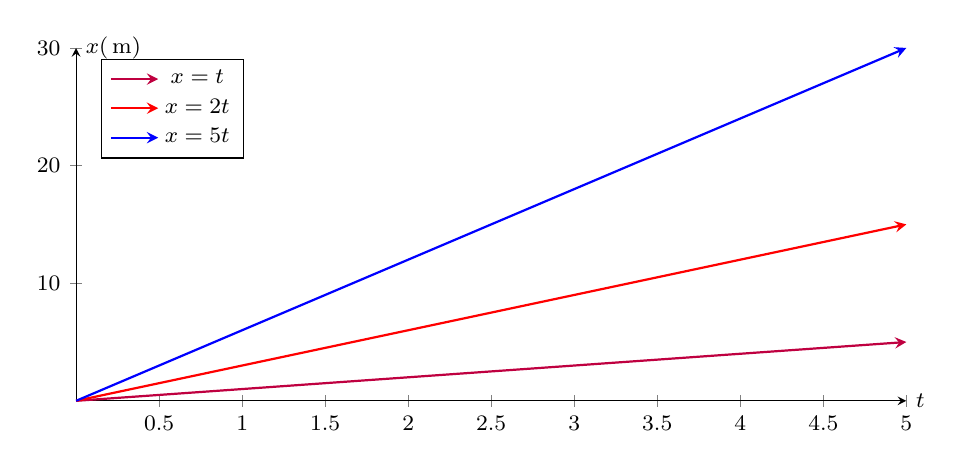
\begin{tikzpicture}
        \begin{axis}[
            my axis style,
            width=\textwidth,
            height=.5\textwidth,
            legend entries={
                $x = t$,
                $x = 2t$,
                $x = 5t$
            },
            legend pos=north west
        ]
        
        \addplot[
            domain=0:5,
            thick,
            purple,
            ->
        ]
        {x};
    
        \addplot[
            domain=0:5,
            thick,
            red,
            ->
        ]
        {3*(x)};
    
        \addplot[
            domain=0:5,
            thick,
            blue,
            ->
        ]
        {6*(x)};
        
        \fill[
            black
        ];
        
        \end{axis}
        \end{tikzpicture}
        \caption{Pos V. Time}
        \label{fig:my-awesome-graph}
    \end{figure}

    \begin{soln}
        \begin{proof}
            We just need to prove that the distance traversed by \textcolor{blue}{Racer $Z$} at the end of the race was more than the other racers. Since the equations of motions are given, we can simply compute the distance traveled by each racer after the end of the race. 
            \begin{align*}
                \textcolor{red}{Racer Y} \colon x &= 2t \\
                &= 2(5) \m\\
                &= 10\m\\
                \textcolor{purple}{Racer X} \colon x &= t \\
                &= (5) \m \\
                &= 5\m \\
                \textcolor{blue}{Racer Z} \colon x &= 5t\\
                &= 5(5) \m \\
                &= 25 \m
            \end{align*}
            Since the distance traveled by \textcolor{blue}{Racer $Z$} is greater than the distance traveled by the other racers by the end of the race, we can conclude that he must of won the race.
        \end{proof}


    \end{soln}



\end{qstn}


\begin{qstn}[5]
A ball is dropped from a cliff $20\m$[North] relative to the ground. The ball bounces off the ground and reaches a final position $15\m$[South] relative to the cliff. The entire trip took $12$ seconds. Determine,
\begin{enumerate}[label = (\alph*)]
    \item The average velocity of the ball
    \item The average speed of the ball
    \item The Pos v. Time plot of the ball
\end{enumerate}

\begin{soln}
    \begin{enumerate}[label = (\alph*)]
        \item \textbf{\underline{Solution 1:}} To determine the average velocity of the ball we must compute $\Delta \vec d$. First we must agree on a reference point to take our measurements from, I will choose the ground. Next I will assign [North] as the positive direction of motion. The initial position vector of the ball relative to the ground is $\vec d_I = +20\m$. To determine the final position vector of the ball will require some relative vector operations, we know the final position of the ball relative to cliff is $\vec d_{\tx{BALL rel CLIFF}} = -15\m$, and we also know $\vec d_{\tx{CLIFF rel GRND}}$. Knowledge of these two position vectors allows us to use proposition 1.6.1, 
        \begin{align*}
            \vec d_{\tx{BALL rel GRND}} &= \vec d_{\tx{BALL rel CLIFF}} + \vec d_{\tx{CLIFF rel GRND}}\\
            &= -15\m + (+20\m)\\
            &= +5\m\\
        \end{align*}
        We can now deduce the average velocity of the ball,
            $$\vec v_{av} = \frac{\Delta \vec d}{\Delta t} = \frac{\vec d_F - \vec d_I}{\Delta t} = \frac{+5 - (+20)}{12} = -\frac{15}{12} \m / \s = \frac{5}{4} \m / \s \tx{[South]}$$\\


        \textbf{\underline{Solution 2:}} In this solution I will only change my reference point and choose the cliff instead, we will continue to call [North] the positive direction of motion. Initally the ball is $\vec d_I = +0 \m$ relative to the cliff and finally the ball is $\vec d_F = -15\m$ relative to the cliff, hence
        $$\vec v_{av} = \frac{\Delta \vec d}{\Delta t} = \frac{-15 - (+0)}{12} = -\frac{5}{4} \m / \s = \frac{5}{4} \m / \s \tx{[South]}$$
        \textbf{(THIS SOLUTION IS WAY EASIER, ALWAYS CHOOSE SMART REF POINT)}
            
        \item To determine the average speed of the ball, we need to compute the total distance traveled by the ball by summing over its displacements. Its first displacement was $\Delta \vec d_1 = 20\m$[S]. Afterwards it traveled from the ground to a position $\vec d_{\tx{BALL rel GRND}} = 5\m$[N] (From (a)), hence its second displacement was $\Delta d_2 = 5\m$ [N]. We apply Corollary 1.2.0.1 to determine the distance traveled,
        \begin{align*}
            d &= \sum_i |\overrightarrow{\Delta d_i}|\\
            &= |\overrightarrow{\Delta d_1}| + |\overrightarrow{\Delta d_2}|\\
            &= |-20\m| + |+5\m|\\
            &= 20\m + 5\m\\
            &= 25\m\\
            v_{av} &= \frac{d}{\Delta t}\\
            &= \frac{25}{12} \m / \s
        \end{align*}
    \end{enumerate}



\end{soln}

\end{qstn}


\begin{qstn}[6]
    A sprinter completes a sprint (returning back to his starting position) in $30$ seconds around a circular track with radius $15\m$. Compute the sprinters,
    \begin{enumerate}[label = (\alph*)]
        \item Average speed
        \item Average velocity
    \end{enumerate}

    \begin{soln}
        \begin{enumerate}[label = (\alph*)]
            \item To determine the average speed we must first compute the total distance traveled by the sprinter during the sprint. This will require us to compute the circumference of the track, 
            \begin{align*}
                d &= 2\pi r\\
                &= 2\pi(15)\\
                &= (30\pi) \m
            \end{align*}
            We can now compute the average speed,
            \begin{align*}
                v_{av} &= \frac{d}{\Delta t}\\
                &= \frac{(30\pi)\m}{30\s}\\
                &= (\pi) \m / s
            \end{align*}
            \item The average velocity of the sprinter must be $+0 \m / \s$ since the sprinter starts and finishes at the same position. ($\Delta \vec d = +0 \m$)
        \end{enumerate}

    \end{soln}


\end{qstn}


\begin{qstn}[7]
    Car $A$ and Car $B$ are about to race each other, however Car $B$ wants to challenge himself by letting car $A$ have a $3$ second head start. If car $A$ has an average speed of $120 \m / \s$, at what average speed must Car $B$ race at in order to tie the race? The length of the race track is $4.2 \km$.



    \begin{soln}
        Let the time it takes for Car $B$ to complete the race be $\Delta t_A$, I claim that the time necessary for Car $B$ to tie the race is $\Delta t_A - 3$. To see why this is true, recall that Car $B$ gives Car $A$ a $3$ second head start, hence the time that Car $A$ will take to complete the remainder of the race after this $3$ second head start is $\Delta t_A - 3$, during this time period Car $A$ must be able to clear the track,
        \begin{align*}
            \Delta t_A &= \frac{d}{v_{av}}\\
            &= \frac{4.2 \km }{120 \m / \s}\\
            &= \frac{4200\m}{120 \m / \s} \tag{4.2\km = 4200\m}\\
            &= 35 \s
        \end{align*}
        We can now compute the necessary average speed for Car $B$ to race at in order to tie the race,
        \begin{align*}
            v_{av} &= \frac{d}{\Delta t_A - 3}\\
            &= \frac{4200\m}{35 \s - 3}\\
            &= \frac{4200 \m}{32}\\
            &= 131.25 \m / \s\\
        \end{align*}

    \end{soln}


\end{qstn}


\begin{qstn}[8]
    The Robetson's Family are interested in doing business with a particular salesmen. They decide to drive over to Toronto to catch him at his bus stop before he departs. Let us suppose that this bus stop is located at $(0,0)$. The Roberston's mistakenly passed this bus stop, not knowing that the salesmen was at this particular one, and only realized they missed him after having traveled to a position $\vec d = +100\m$ relative to the bus stop, at an average speed of $60 \m / \s$. The \emph{exact} moment they passed him was the moment that his bus started to travel in a direction [West] relative to the bust stop at an average velocity of $50 \m / \s $[\tx{West}]. If at the exact moment the Robertson's had reached the position $\vec d = +100\m$, the salesmen got off at his next stop, at what speed must the Roberston's travel at in order to catch up to him within $30$ seconds?


    \begin{soln}
        In this problem we must keep track of the position of both the Roberston's as well as the salesmen. Let us assign the [East] direction as the positive direction of motion. Let the Roberston's be labeled by the variable $R$, and the Salesmen be labeled $S$. 

        

    \begin{center}
        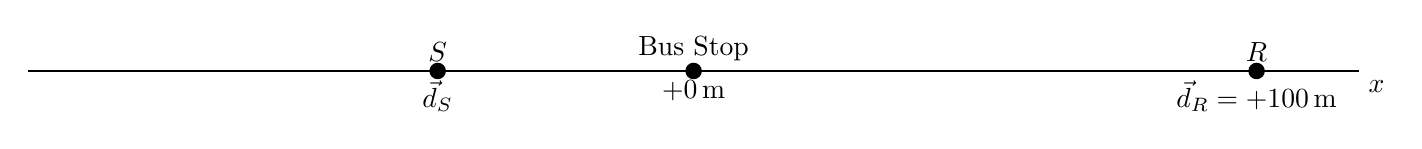
\begin{tikzpicture}[scale=0.65]%
        \draw [-] (26,0) node[below right]{$x$} -- (0,0) -- (26,0);

        \node [above] at (13,0) {$\tx{Bus Stop}$};
        \node [below] at (13,0) {$+0\m$};
        \draw[fill=black] (13,0) circle(1.5mm);

        \node [below] at (24,0) {$\vec d_R = +100\m$};
        \node [above] at (24,0) {$R$};
        \draw[fill=black] (24,0) circle(1.5mm);

        \node [below] at (8,0) {$\vec d_S$};
        \node [above] at (8,0) {$S$};
        \draw[fill=black] (8,0) circle(1.5mm);

        \end{tikzpicture}
    \end{center}

    \textbf{Note : }Throughout the remainder of this problem, it is not nessecarry to continue operations with the vector quantities, instead we can work with distances and speeds, the vector quantities merely allow us to depict the diagram above to understand the motion of both the Salesmen and the Robertson's.\\

    We need to compute the position vector $\vec d_S$ of the Salesmen after the Robertsons have traveled to a position $\vec d_R = +100\m$. To compute this position vector, recall that the moment that the Robertsons reach the position $\vec d_R = +100\m$, the Salesmen has departed from his bus and has reached the position $\vec d_S$. Hence we must compute the time,$\Delta t_1$, taken for the Roberston's to reach the position vector $\vec d_R$, in this amount of time we can compute the position of the Salesmen.
    \begin{align*}
        \Delta t_1 &= \frac{d_R}{v_{av}}\\
        &= \frac{100\m}{60\m / \s}\\
        &= \frac{5}{3} \s
    \end{align*}
    During this time $\Delta t_1$, the Salesmen must of traveled a westward distance,
    \begin{align*}
        d_S &= (v_{av})(\Delta t_1)\\
        &= (50 \m / \s)(\frac{5}{3} \s)\\
        &= \frac{50 \cdot 5}{3}\m \\
        &= 83.33\m
    \end{align*}
    Let the distance from $R$ to $S$ be denoted $d_{RS} = d_R + d_S = 100 + 83.33 = 183.33$. This is the distance that the Robertson's must travel within $30\s$ in order to reach the Salesmen. Hence we can compute the required speed,
    \begin{align*}
        v_{av} &= \frac{d_{RS}}{\Delta t}\\
        &= \frac{183.33\m}{30\s}\\
        &= 6.11 \m / \s
    \end{align*}
    Hence the required speed for the Roberston's is $v_{av} = 6.11 \m / \s$.


    \end{soln}


    \end{qstn}

    







\end{document}
%   \begin{figure}[H]
%   \centering
%   \includegraphics[width=0.75\linewidth]{p}
%   \caption{caption.\label{fig:}}
%   \end{figure}























